% Set the author and title of the compiled pdf
\hypersetup{
	pdftitle = {\Title},
	pdfauthor = {\Author}
}

\section{Functions}

A mathematical function is a relation between a set of inputs and a set of
outputs. Each input is related to exactly one output, and the same input will
{\it always} result in the same output.

\subsection{Simple functions}

Functions can be split into three components; a source, a target and the
behaviour of the function.

The source and target of a function are both sets, and are denoted as $S$ and
$T$ respectively in the following notation:

\[
	f:S \rightarrow T
\]

In order to find the value of a function $f$ for a specific input $x$, the
notation is:

\[
	f(x)
\]

Describing the behaviour of a function requires another notation:

\[
	x \longmapsto \dots x \dots
\]

Consequently, to completely describe a function by defining its source, target
and behaviour, we must write something like:

\[
	\begin{split}
	f:S &\rightarrow T\\
	x &\longmapsto \dots x \dots
	\end{split}
\]

An example of this may be a function that finds the absolute value of integers:

\[
	\begin{split}
	abs:\mathbb{Z} &\rightarrow \mathbb{N}\\
	x &\longmapsto |x|
	\end{split}	
\]

\subsection{Equality of functions}

Two functions are said to be equal to each other if the following conditions are
met:

\begin{itemize}
	\item The source set is the same
	\item The target set is the same
	\item The behaviour of the functions is the same (so for every $x \in S$, 
		  where $S$ is the source set, both functions give the same output $y$
		  when given $x$ as the input, where $y \in T$ and $T$ is the target
		  set).
\end{itemize}

\subsection{Identity functions}

For any set $S$, there is a function such that:

\[
	\begin{split}
	f:S \rightarrow S\\
	x \longmapsto x
	\end{split}
\]	

This is described as the identity function of $S$, and is often denoted by $1_S$
or $id_S$

\subsection{Injectivity, Surjectivity and Bijectivity}

The terms {\it injective}, {\it surjective} and {\it bijective} are used to
describe which elements in a functions source set are mapped to which elements
its target set:

\begin{description}
	\item {\bf Injective}\\
		For each $x \in S$ there is at most one $y \in T$ such that $f(x) = y$.
	\item {\bf Surjective}\\
		For each $x \in S$ there is at least one $y \in T$ such that $f(x) = y$.
	\item {\bf Bijective}\\
		For each $x \in S$ there is only one $y \in T$ such that $f(x) = y$.
\end{description}

Note that if an function is injective and surjective, then it must also be
bijective.

\subsubsection{Permutation of sets}

A function is said to be a permutation of a set if the source and target of the
function is the same set and the function is bijective. Applying the function
effectively re-arranges the members of the set.

\subsection{Function composition}

Two functions can be composited when the source set of one function is the same
as the target set of another. For example:

\[
	\begin{split}
		f:S \rightarrow T\\
		g:T \rightarrow U
	\end{split}
\]

Here, we can compose a new function made up of $f$ and $g$:

\[
	h = g \circ f
\]

Or in other words:

\[
	h(x) = g(f(x))
\]

When we're invoking composition on more than two functions, it is an associative
operation. For this reason, we often omit brackets and the circle operator:

\[
	(f \circ (g \circ h)) = fgh
\]

\subsection*{Functions with recursive definitions}

If a function references itself in its own body, then it is recursive. An
example might be:

\[
	\begin{split}
		&f:\mathbb{N} \rightarrow \mathbb{N}\\
		f(0) &= 0\\
		f(r + 1) &= f(r) + 1
	\end{split}
\]

This function just returns the input it is given, but the 

\section{Induction}

Induction is a technique that allows us to use the property of infinite
countability of natural numbers ($\mathbb{N}$) to prove theorems.

Induction works by defining a {\bf base case}, where some iterative variable
(usually $n$) is equal to $0$, and then coming up with a {\bf step case}, that
says when you add $1$ to $n$ for any $n$, then the result is also true. Since
natural numbers are infinitely countable, then the step case must hold for all
$n$.

\subsection{Induction example}

The most basic example of induction is to prove something like:

\begin{align*}
	&\forall n \in \mathbb{N}\\
	&0 + 1 + 2 + \dots + n = \frac{n(n + 1)}{2}
\end{align*}

\begin{description}
	\item {\bf Base case}:\\
		When $n = 0$ both sides of the equation equal $0$.
	\item {\bf Step case}:\\
		In order to prove the step case, we should first assign names to both equations:
		\[
			\begin{split}
				L(n) &= 0 + 1 + 2 + \dots + n\\
				R(n) &= \frac{n(n + 1)}{2}
			\end{split}
		\]
		
		Now, if we assume that $L(n) = R(n)$ as it is in the base case, we now
		need to prove that $L(n+1) = R(n+1)$:

		\[
			\begin{split}
				L(n + 1) 						 &= L(n) + (n+1)\\
												 &= R(n) + (n + 1)\\
												 &= \frac{n(n + 1)}{2}(n + 1)\\
												 &= \frac{n(n + 1) + 2(n + 1)}{2}\\
												 &= \frac{n(n + 1) + 2n + 2)}{2}\\
												 &= \frac{n^2 + n + 2n + 2)}{2}\\
												 &= \frac{n^2 + 3n + 2)}{2}\\
												 &= \frac{n^2 + 3n + 2)}{2}\\
												 &= \frac{(n + 2)(n + 1)}{2}\\
												 &= R(n+1)
			\end{split}
		\]
\end{description}


\subsection*{Summation notation}

Often, you will be asked to provide an inductive proof for an equality where one
side of the equation is a summation. The syntax is like so:

\[
	\sum\limits^n_{i=0} i
\]

This is the notation for adding all the numbers from $0$ to $n$, like:

\[
	0 + 1 + 2 + \dots + n
\]

The number above the sigma is the limit of the summation, and the number below
is the starting value.

Forming inductive proofs with this notation isn't much different to doing it
without. All you do is add $1$ to all the instances of your inductive variable
and then rearrange the equation to get the other side.

\subsubsection*{An inductive proof of a summation}

Lets prove that:
\[
	\sum\limits^n_{i=0} x^i = \frac{x^{n-1} - 1}{x - 1}
\]

So first, we have that:

\[
	\begin{split}
		L(n) &= \sum\limits^n_{i=0} x^i\\
		R(n) &= \frac{x^{n-1} - 1}{x - 1}
	\end{split}
\]

First, lets prove the base case, when $n=0$:

\[
	\begin{split}
		L(0) = x^0 = 1\\
		R(0) = \frac{-1}{-1} = 1
	\end{split}
\]

Now, we can prove the step case:

\[
	\begin{split}
		L(n + 1) &= L(n) + x^{n+1}\\
				 &= R(n) + x^{n+1}\\
				 &= \frac{x^{n-1} - 1}{x - 1} + x^{n+1}\\
				 &= \frac{x^{n-1} - 1 + (x - 1)(x^{n+1})}{x - 1}\\
				 &= \frac{x^{n-1} - 1 + x^{n} - x^{n - 1}}{x - 1}\\
				 &= \frac{x^{n} - 1}{x - 1}\\
				 &= R(n+1)
	\end{split}
\]

\section{Relations}

A relation is a set of pairs between two sets. You can think of it as a subset
of the powerset of two sets. For example, if we have a relation $R$ between the
numbers $\{1,2,3\}$ and $\{4,5,6\}$, where the even and odd numbers are paired
together, then it will look like this:

\[
	\begin{split}
		A &= \{1,2,3\}\\
		B &= \{4,5,6\}\\
		A \times B &= \begin{Bmatrix}
						(1,4)&(1,5)&(1,6)\\
						(2,4)&(2,5)&(2,6)\\
						(3,4)&(3,5)&(3,6)
					  \end{Bmatrix}\\
		R \subset (A \times B) &= \begin{Bmatrix}
									(1,5)\\
									(2,4)&(2,6)\\
									(3,5)
								 \end{Bmatrix}
	\end{split}
\]

If we want to represent that an element $a \in A$ is related to an element $b
\in B$ via a relation $R$, then we write $aRb$.

Obviously, relations aren't related to natural numbers as in the previous
example. You can have a relation between sets of any type. For example, you
could define a relation between family members. The relation $P$ could hold when
an element $a$ is the father of another element $b$.

If you can define a relation between family members, then it makes sense that
you should also be able to draw a diagram like a family tree then. Such graphs
are called {\it digraphs}, they might look like this:

\begin{center}
  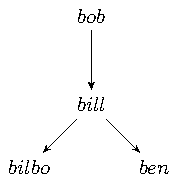
\includegraphics{digraphs/1.pdf}
\end{center}

From this digraph, we can see that $bill~R~bilbo$, $bill~R~ben$ and
$bob~R~bill$.

\subsection{Properties of relations}

We can describe relations as possessing different properties; the four properties
we cover in this course are as follows:

\begin{description}
	\item {\bf Reflexive}:\\
		A relation is reflexive if all the elements in the relation have a
		relation to themselves. In mathematical terms:
		\[
			a \in A~then~aRa
		\]
	\item {\bf Symmetric}:\\
		If a relation is symmetric, then if two elements are related, then the
		relation must go both ways. In other words:
		\[
			(a,b) \in A~then~aRb \implies bRa
		\]
	\item {\bf Antisymmetric}:\\
		A relation that is antisymmetric, then no relations work both ways. An
		example of an antisymmetric relation is the father relation we defined
		before; it is impossible for two distinct elements to be each others
		father. Mathematically, 
		\[
			(a,b) \in A~then~(aRb \wedge bRa) \implies a=b
		\]
	\item {\bf Transitive}:\\
		A transitive relation is one where if an element $a$ is related to
		another element $b$, and $b$ is related to $c$, then $a$ must be related
		to $c$:
		\[
			(a,b,c) \in A~then~(aRb \wedge bRc) \implies aRc
		\]
\end{description}

\subsection{Equivalence relation}

A relation is said to be an equivalence relation if it is reflexive, symmetric
and transitive. The idea is that if $R$ is an equivalence relation, then if
$aRb$, then in some sense, $a$ and $b$ are the same.

An equivalence relation splits a set into a number of partitions. Each partition
is made up of elements of the set that are equivalent to each other. An {\it
equivalence class} is a subset of elements in the set that are equivalent to
each other as previously described. The notation for an equivalence class is
$[a]_R$, where all the elements in that equivalence class will be related to
$a$ under the relation $R$.

\marginpar{Sometimes the subscript $R$ is missed off the notation for
equivalence classes if the relation in question is clear from the context; i.e.
you could write $[a]$ instead of $[a]_R$.}

If we were to take the set of natural numbers $\mathbb{N}$ and define the $R$ so
that $aRb$ if $a$ and $b$ are both even or both odd. This would mean that
$\mathbb{N}$ would be split into two equivalence classes, that would form a
partition, for example, $\mathbb{N} = [2] \cup [7]$.

Mathematically, these are the principles of equivalence relations and
equivalence classes:

\begin{itemize}
	\item $a \in [a]$
	\item $b,c \in [a]_R \implies bRc$
	\item For any $a,b$ either $[a] = [b]$ or $[a] \cap [b] = \emptyset$
\end{itemize}

\subsection{Operations on Relations}

Just like sets, you can perform operations such as union and intersection on
relations. They are easily defined in a mathematical sense:

\begin{description}
	\item {\bf Union}\\
		In order to create a new relation $Z$ that is the union of the two
		relations $X$ and $Y$, you would do:
		\[
			Z = X \cup Y = \{(a,b) \in Z | (a,b) \in X \vee (a,b) \in Y\}
		\]

		An example might be if you take the union of the `{\it is father of}'
		relation and the `{\it is mother of}' relation, then you'll get an `{\it
		is parent of}' relation.

	\item {\bf Intersection}\\
		Similar to the union, except you use an {\tt and} operator instead of an
		{\tt or}:
		\[
			Z = X \cap Y = \{(a,b) \in Z | (a,b) \in X \wedge (a,b) \in Y\}
		\]

		An example might be if you take the intersection of the relation `{\it
		person resides in Ali G}' and `{\it doesn't go to Manchester
		University}', you'd get a relation describing lots of rather suspicious
		looking Man Met students.

	\item {\bf Complement}\\
		To find the complement of a relation, you just define another relation
		based on the pairs not defined in the first one:
		\[
			Z = X^c = \{(a,b) \in Z | (a,b) \not\in X\}
		\]

		A complement operation would have the effect of transforming the
		relation `{\it are married}' to `{\it not married}'.

	\item {\bf Inverse}\\
		The inverse of a relation is where the direction of all the arrows on
		the digraph are reversed:
		\[
			Z = X^{-1} = \{(a,b) \in Z | (b,a) \in X\}
		\]

		Inverting the relation `{\it is older than}' would yield an `{\it is
		younger than}' relation.

\end{description}

\subsection{Relational composition}

If one relation ($R_1$) is defined from $A$ to $B$ and another ($R_2$) from $B$
to $C$, then it is possible to define a third relation that is composed of the
first two that is defined from $A$ to $C$. This is relational composition:

\[
	R_2 \circ R_1 = \{(a,c) \in A \times C | \exists b \in B, (a,b) \in R_1 \wedge (b,c) \in R_2 \}
\]

\marginpar{Note the order of the operands here}

\subsection{P Closures}

In terms of relations, a $P$ Closure is constructed when you add the minimum
number of pairs to a relation in order to give the relation the specific
property $P$. For example, the transitive closure of a relation $R$ is a new
relation based on $R$, but with all the extra pairs (which could be no extras)
required to make the relation transitive.

If $P$ is reflexive, symmetric or transitive, then a closure can {\it always} be
constructed.

\subsection{Ordered sets}

A {\it partial order} is a transitive, anti-symmetric and reflexive relation. A
partially ordered set (aka {\it poset}) is a set together with a partial order.
One example of this the the set of integers $\mathbb{Z}$, which when taken
together with the operator `$\geq$' becomes a partially ordered set, since any
integer in the set can be compared to any other integer in the set.

A partial order that can compare {\it any element} is referred to as a total
order.

\subsubsection{Maximal and minimal elements}

A minimal element $m$ of a poset $X$ with a partial ordering \guilsinglleft~
is one where:

\[
	\forall a \in X, m~\textrm{\guilsinglleft}~a
\]

A maximal element is similar:


\[
	\forall a \in X, a~\textrm{\guilsinglleft}~m
\]
